% THIS IS AN EXAMPLE DOCUMENT FOR VLDB 2012
% based on ACM SIGPROC-SP.TEX VERSION 2.7
% Modified by  Gerald Weber <gerald@cs.auckland.ac.nz>
% Removed the requirement to include *bbl file in here. (AhmetSacan, Sep2012)
% Fixed the equation on page 3 to prevent line overflow. (AhmetSacan, Sep2012)

\documentclass{vldb}
\usepackage{graphicx}
\usepackage{balance}  % for  \balance command ON LAST PAGE  (only there!)


\begin{document}

% ****************** TITLE ****************************************

\title{Optimisation of an embedded sensor fusion for 3D positioning}

% possible, but not really needed or used for PVLDB:
%\subtitle{[Extended Abstract]
%\titlenote{A full version of this paper is available as\textit{Author's Guide to Preparing ACM SIG Proceedings Using \LaTeX$2_\epsilon$\ and BibTeX} at \texttt{www.acm.org/eaddress.htm}}}

% ****************** AUTHORS **************************************

% You need the command \numberofauthors to handle the 'placement
% and alignment' of the authors beneath the title.
%
% For aesthetic reasons, we recommend 'three authors at a time'
% i.e. three 'name/affiliation blocks' be placed beneath the title.
%
% NOTE: You are NOT restricted in how many 'rows' of
% "name/affiliations" may appear. We just ask that you restrict
% the number of 'columns' to three.
%
% Because of the available 'opening page real-estate'
% we ask you to refrain from putting more than six authors
% (two rows with three columns) beneath the article title.
% More than six makes the first-page appear very cluttered indeed.
%
% Use the \alignauthor commands to handle the names
% and affiliations for an 'aesthetic maximum' of six authors.
% Add names, affiliations, addresses for
% the seventh etc. author(s) as the argument for the
% \additionalauthors command.
% These 'additional authors' will be output/set for you
% without further effort on your part as the last section in
% the body of your article BEFORE References or any Appendices.

\numberofauthors{2} %  in this sample file, there are a *total*
% of EIGHT authors. SIX appear on the 'first-page' (for formatting
% reasons) and the remaining two appear in the \additionalauthors section.

\author{
% You can go ahead and credit any number of authors here,
% e.g. one 'row of three' or two rows (consisting of one row of three
% and a second row of one, two or three).
%
% The command \alignauthor (no curly braces needed) should
% precede each author name, affiliation/snail-mail address and
% e-mail address. Additionally, tag each line of
% affiliation/address with \affaddr, and tag the
% e-mail address with \email.
%
% 1st. author
\alignauthor
ASGHARI Seyed Amir\\
       \affaddr{Sorbonne University, Engineering faculty}\\
       \affaddr{Paris, France}\\
       \email{amirsinasghari@gmail.com}
% 2nd. author
\alignauthor
PONCELET Renaud\\
       \affaddr{Sorbonne University, Engineering faculty}\\
       \affaddr{Paris, France}\\
       \email{renaud.poncelet@gmail.com}
% 3rd. author
\and
\alignauthor BALDE Hamidou\\
       \affaddr{Sorbonne University, Engineering faculty}\\
       \affaddr{Paris, France}\\
       \email{hamidou2balde@yahoo.fr}
% use '\and' if you need 'another row' of author names
% 4th. author
\alignauthor CAGLAYAN Ibrahim\\
       \affaddr{Sorbonne University, Engineering faculty}\\
       \affaddr{Paris, France}\\
       \email{ibrahimcag94@gmail.com}
}



\maketitle

\begin{abstract}
Nowadays, we can find different sensors which enable to position a real object in a virtual word. Almost all of them are big, expensive and not always efficient (occlusion or luminosity issues). In many cases, sensors have qualities and defaults. The most representative example is the the fast but imprecise sensor or the slow but precise one. However by combining many of them, we can get rid of the defaults and keep only the qualities. The objective is to create a sensor fusion algorithm to enable compact, cheap and efficient 3d positioning.
\end{abstract}




\section{INTRODUCTION}
This article is the continuation of \cite{cedric}, where the whole project has been initiate and developed. This article provide the simulation of the presented project that will also be presented here. \newline
There are many techniques for 3D positioning. Firstly, some technique uses multiple camera setup like in \cite{lee2013real}, where they detect and track an object by using the geometry between the target object and cameras to finally provide a 3D positioning of the object. The main contribution was the refinement stage that correct detection and tracking error by imposing geometric constrain. However, the setup is long and cannot be made in any room quickly. \newline
Then, some are using this visual information with inertial information in order to fusion the data like in \cite{bleser2009advanced} using the principle of data fusion as described in \cite{chair1986optimal}, where they each decision is weighted according to the reliability i.e the precision of the detectors. In this configuration, they rely on a 3D model of the scene that enables to predict the appearances of the features by rendering the model using the prediction data of the
sensor fusion filter. Their paper presented a markerless vision-inertial tracking system that works in small and large scale rooms, with good or bad luminosity. The final system is efficient and robust but one of the main issue of this kind of application is the cost of the cameras.\newline
This paper is focus on another principle that is inspired from the HTC Vive. This technique uses light house scanning to track the object as in \cite{kreylos2016lighthouse}. This article will firstly explain the lighthouse operating principle in section 2. Then, it will explain the hive track operating principle in section 3. Thereafter, it will present the modelling and the simulation made to test the sensor fusion for 3D positioning in section 4 and finally it will present the results in section 5. This paper is related to the project : https://hivetracker.github.io, and it also have his own project github at \newline https://github.com/VR3Dtracking.



\section{Operating principle}
The lighthouse tracking system uses the principle of triangulation to position an object. This technique can be used to approximate the distance between two point that cannot be measured like it's shown in figure [\ref{plage}], where the two person can measure the distance of the rock by knowing the distance between each others and their angle when they look at the stone.
\begin{figure}
\centering
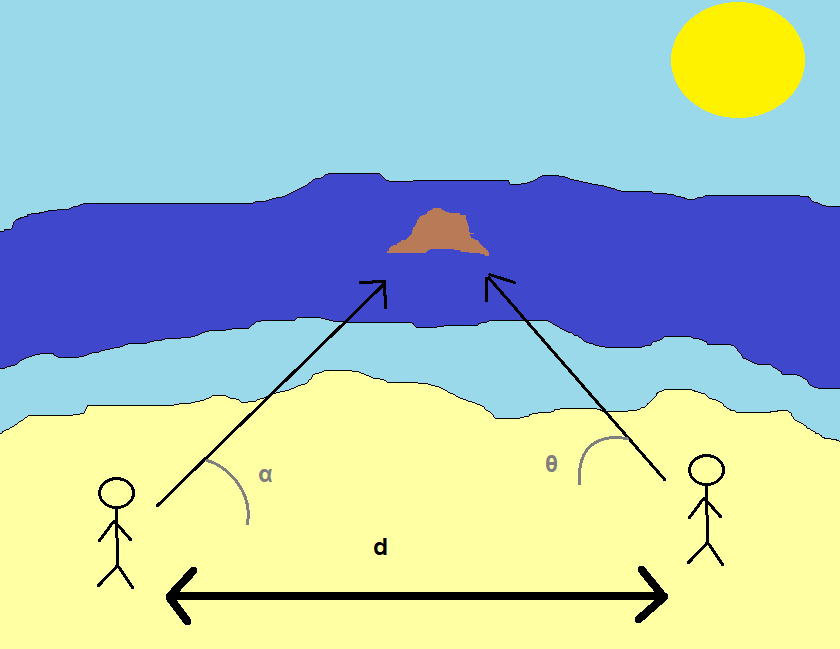
\includegraphics[scale=0.35]{Image/plage.png}
\caption{Illustration of the use of the triangulation method, two person look at a rock and obtain an approximate angle between their gaze and the other person $\alpha$ and $\beta$. Then, knowing the distance $d$ between each others, the distance between the beach and the rock can get measured.}
\label{plage}
\end{figure}
The lighthouse system is the same, but it's done in 3 dimension. So its main objective is to obtain four angles to be able to compute the position of an object. 
There are some requirement for positioning an object by using the light House. First, a room needs to be defined where the object can be tracked only in this space. Then, the object needs to have photo-diodes on him, because the lighthouse will emit infra red light (that can be presented by a laser) and get the value of the angle from the data of the photo-diode. Finally, the two lighthouses needs to be synchronized in order to have workable values.
\bigbreak
\begin{figure}
\centering
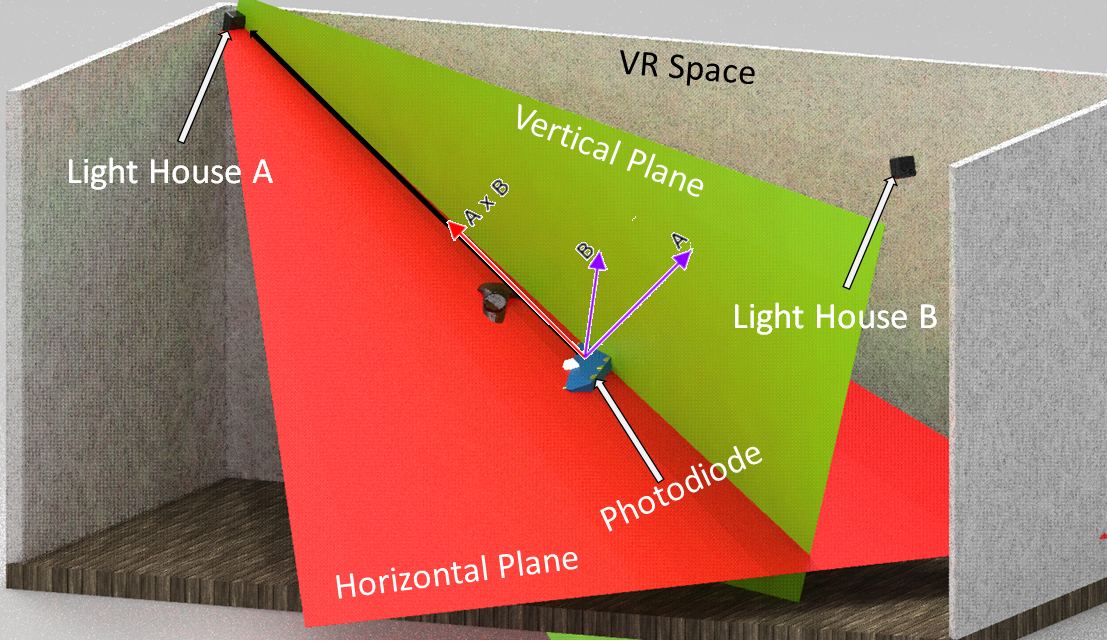
\includegraphics[width=1.0\columnwidth]{Image/LH1.png}
\caption{Demonstration of a lighthouse positioning system, where the two scanning plan (horizontal and vertical), in red and green can be seen \cite{cedric}}
\label{plage}
\end{figure}
This is how the system works: two (or more) lighthouses will be positioned on the opposite corner of the room. The object, that have a photo-diode on it, will be in this room. One of the lighthouse (Lighthouse A) will emit a flash that the photo-diode will receive. Then it will sweep a laser plan left to right (vertically). After it scanned half a period, it will emit another flash and then sweep another laser plan down to top (horizontally) for another half a period. The other lighthouse (lighthouse B) will do exactly the same right after the horizontal sweeping of the first lighthouse. After this, the value of the photo-diode throw time will be like figure [\ref{photo}].
\begin{figure}
\centering
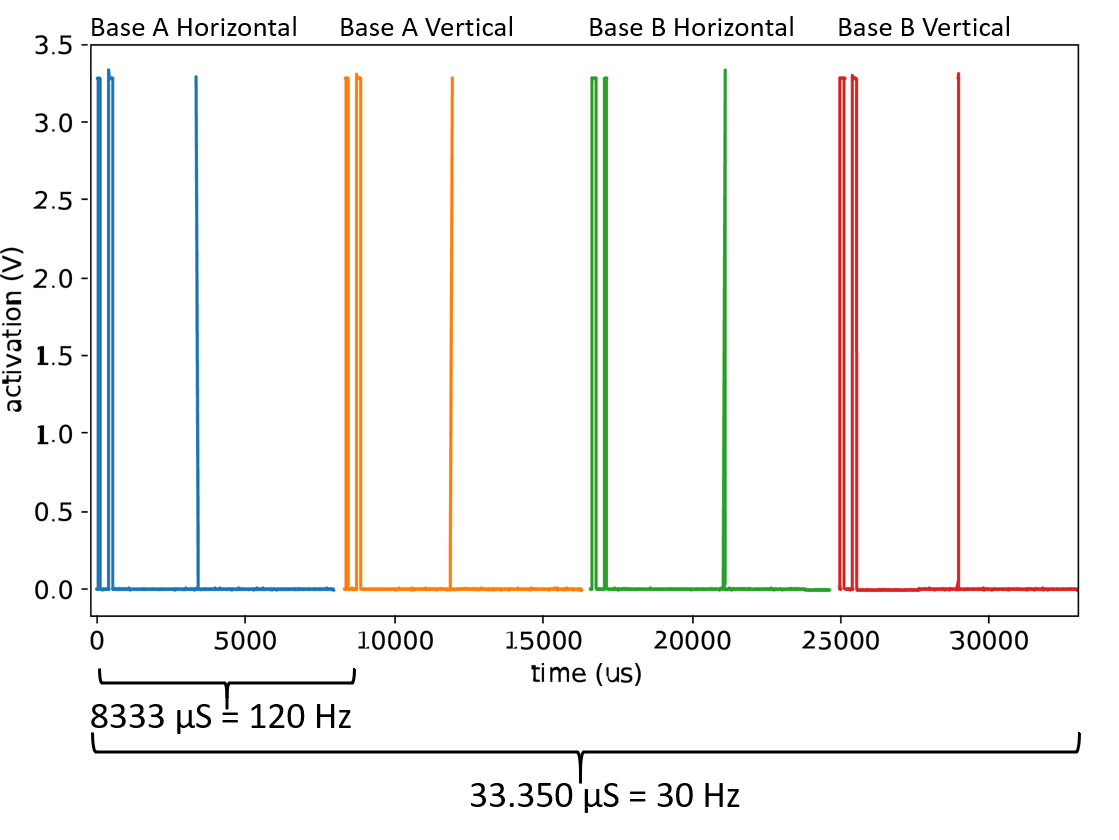
\includegraphics[width=1.0\columnwidth]{Image/Signal2.png}
\caption{Light signal sequences (4 are shown): wide pulses are base station flashes and short pulses are laser plane scans. One lighthouse takes 8.3333 $\mu$seconds to sweep a semi-period, therefor, a complete positioning takes about 35 $\mu$seconds \cite{cedric}}
\label{photo}
\end{figure}
The lighthouse requires $8.333 \mu s$ to sweep a semi-period, a total of $33.333 \mu s$ is therefor required for a full positioning.
Time is therefor a critical information to get the angles that can be get by doing a simple proportional ratio. However, to avoid any confusion for the following calculus, it is mandatory to define a clear and precise landmark for the room and the lighthouses.
\bigbreak
Figure [\ref{box}] shows the landmark of the word as it will be used for the following parts, and figure [\ref{lighthouse}] shows the one of a lighthouse. As it can be seen, the vertical sweep will start from $z$ positive, pass by $y$ positive and ends in $z$ negative. For the horizontal sweep, it will start at $x$ negative, pass by $y$ positive too and ends in $x$ positive. For example, if the object is in the y axis, both sweeping will detect the object at the middle of their sweeping. \newline
\begin{figure}
\centering
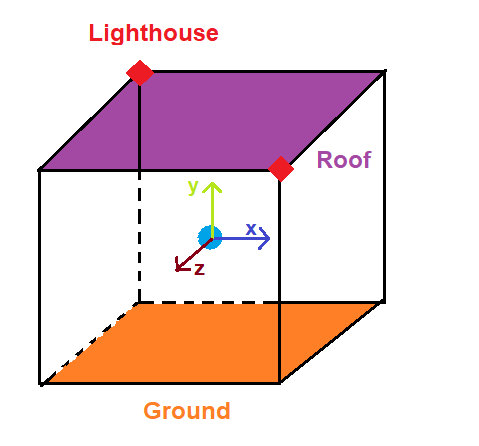
\includegraphics[width=1.0\columnwidth]{Image/box.png}
\caption{A modeling of the room and it's landmark. The box represent the Room, the roof is represented in purple, and the two lighthouses are positioned in the opposite corner of the room. The ground is represented in orange and the landmark positioned in the middle of the box is the Landmark of the world. In this case, if the box cube with a dimension of 1, then the two lighthouses are positioned in (-0.5,0.5,-0.5) and (0.5,0.5,0.5)}
\label{box}
\end{figure}
\begin{figure}
\centering
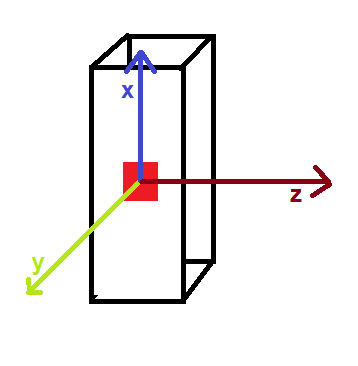
\includegraphics[width=0.6\columnwidth]{Image/lighthouse.png}
\caption{A modeling of the lighthouse and its landmark, the landmark is positioned where the laser is emitted. The direction vector of the sweeping plan when the lighthouse does the horizontal sweep starts at $+z$ and ends at $-z$ passing by $y$. The direction vector of the sweeping plan when the lighthouse does the horizontal sweep starts at $-x$ and ends at $+x$ passing also by $y$ }
\label{lighthouse}
\end{figure}
If this method can detect the object everywhere one the box, there is one line where the object cannot be positioned and this line is the one between the two lighthouses. to be able to eliminate the ambiguity, a third lighthouse will be needed. However, since this line is one the roof of the room, this issue can be ignored (figure [\ref{bad}])
\begin{figure}
\centering
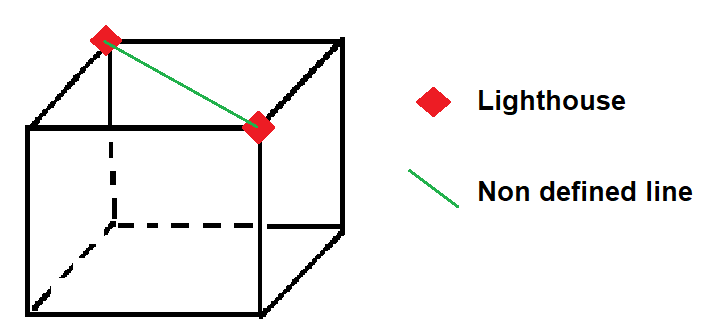
\includegraphics[width=1.0\columnwidth]{Image/boxundefined.png}
\caption{The line where the object cannot be positioned. The black box represents the room and the lighthouses with the red squares. Since the triangulation uses the intersection of two lines, it can't find a point of intersection when the two lines are mixed. The line on witch the position of the object cannot be detected is the green one}
\label{bad}
\end{figure}


\section{Hive track operating principle}
\label{Hive}

The objective is to use the position given by the light house system that it is precise but with a slow rate and the data from the MEMS (Microelectromechanical systems) sensors from the IMU (Inertial measurement unit) which are less precise but with a fast rate and process data fusion in order to have a faster rate and a good precision. Kalman filter is using to realize this data fusion. First, let's define the state system for a 6 DOF (degrees of freedom) object. The following explanations are adapted from \cite{caron2006gps}, but it is actually classical kalman filter application. The state is :
\begin{equation}
\mathbf{X} = 
\begin{pmatrix}
\begin{pmatrix}
x & \frac{dx}{dt} & \frac{d^2x}{dt^2} & \alpha & \frac{d\alpha}{dt}
\end{pmatrix} ^T \\
\begin{pmatrix}
y & \frac{dy}{dt} & \frac{d^2y}{dt^2} & \beta & \frac{d\beta}{dt}
\end{pmatrix} ^T \\
\begin{pmatrix}
z & \frac{dz}{dt} &  \frac{d^2z}{dt^2} & \gamma & \frac{d\gamma}{dt}
\end{pmatrix} ^T
\end{pmatrix}
\end{equation}
note $dt$ the time elapsed since the last estimate. Then for an instant $k$ the estimate at $k+1$ is : 
\begin{equation}
\mathbf{X}(k+1) = A \mathbf{X}(k) +  \mathbf{w}(k)
\end{equation}
with $$\mathbf{A}=
\begin{pmatrix}
\begin{matrix}
\mathbf{F}
\end{matrix} &
\begin{matrix}
\mathbf{0_{5 \times 5}}
\end{matrix} &
\begin{matrix}
\mathbf{0_{5 \times 5}}
\end{matrix} \\
\begin{matrix}
\mathbf{0_{5 \times 5}}
\end{matrix} &
\begin{matrix}
\mathbf{F}
\end{matrix} &
\begin{matrix}
\mathbf{0_{5 \times 5}}
\end{matrix} \\
\begin{matrix}
\mathbf{0_{5 \times 5}}
\end{matrix} &
\begin{matrix}
\mathbf{0_{5 \times 5}}
\end{matrix} &
\begin{matrix}
\mathbf{F}
\end{matrix}
\end{pmatrix}$$
and $\mathbf{w}$ a zero mean white gaussian noise of assumed known covariance matrix $$ \mathbf{Q}(k) = E[ \mathbf{w}(k) \mathbf{w}(k)^T].$$ For  this 6 DOF object let's assume that $$\mathbf{F}=
\begin{pmatrix}
1 & dt & \frac{dt^2}{2} & 0 & 0 \\
0 & 1 & dt & 0 & 0 \\
0 & 0 & 1 & 0 & 0 \\
0 & 0 & 0 & 1 & dt \\
0 & 0 & 0 & 0 & 1 \\
\end{pmatrix}$$.  This model allows to estimate the next state from the actual state. Actually, that's obviously not enough to have a good estimation if $dt$ becames to big or if the model can't rectify his state from a measurement. The kalman filter can rectify the state from a measurement 
\begin{equation}
\mathbf{y}(k) = \mathbf{C} \mathbf{X}(k) + \mathbf{b}(k)
\end{equation} where $ \mathbf{C}$ is the measurement matrix and $\mathbf{b}$ is a white gaussian observation noise with zero mean and with assumed known covariance matrix
\begin{equation}
\mathbf{R}(k) = E[ \mathbf{b}(k) \mathbf{b}(k)^T]
\end{equation} The matrix $\mathbf{C}$ depends on the sensor which feeding the kalman filter. For no measurement $\mathbf{C} = \mathbf{0_{12 \times 12}}$, for a measurement the matrix $\mathbf{C}$ have ones corresponding to each measurements. With this feeding from measurements the state can be evaluated as :
\begin{equation}
 \begin{matrix}
\hat{\mathbf{x}}(k|k) = \hat{\mathbf{x}}(k|k-1) +\\ \mathbf{K}(k)[\mathbf{y}(k)-\mathbf{C}\hat{\mathbf{x}}(k|k-1)]
\end{matrix}   
\end{equation}
 where $\mathbf{K}$ is the kalman gain. There is many integration of kalman filter on c++ language. In our case, $dt$ is not a constant. It depends on many factors like the final rate we want for kalaman estimation, also it depends on the measurement rate which is chaotic because of the using of several sensors and also because of the occlusions which destroy measurements. All this constraints can easily be manage in c++ by using an object which contains all the kalman filter information. Then, the algorithm can update the filter depends on the case : \\ - update without measurement \\ - update with positions measurements from the LEDs and light house system \\ - update with measurements from the IMU

\section{Modelling \& simulation}
\label{Sim}


%GUI presentation

For the simulation the model presented in section 3 has been simplified. In order to have concrete results in a short time the measurements has been reduced to the positions from the LEDs/light house system and to the accelerations from the IMU. All this measurements are actually computed measurements in simulation. Let's explain how this computed measurements have been generated.

\subsection{Graphical User Interface}
\label{GUI}
The objective of the simulation is to first create a 3D model for a better visualization, and then to provide pre-measurements of what can be expected from real data. The GUI for Graphical User Interface can do both. The room is represented by a box, the LightHouses by two sphere on the two top corners and the object by a sphere initialy at the center. The scanning is represented by colored spheres turning around the LightHouses. These spheres actually represent the normal vector of the plan of the scanning as explained in section 2. \newline
\begin{figure}
\centering
    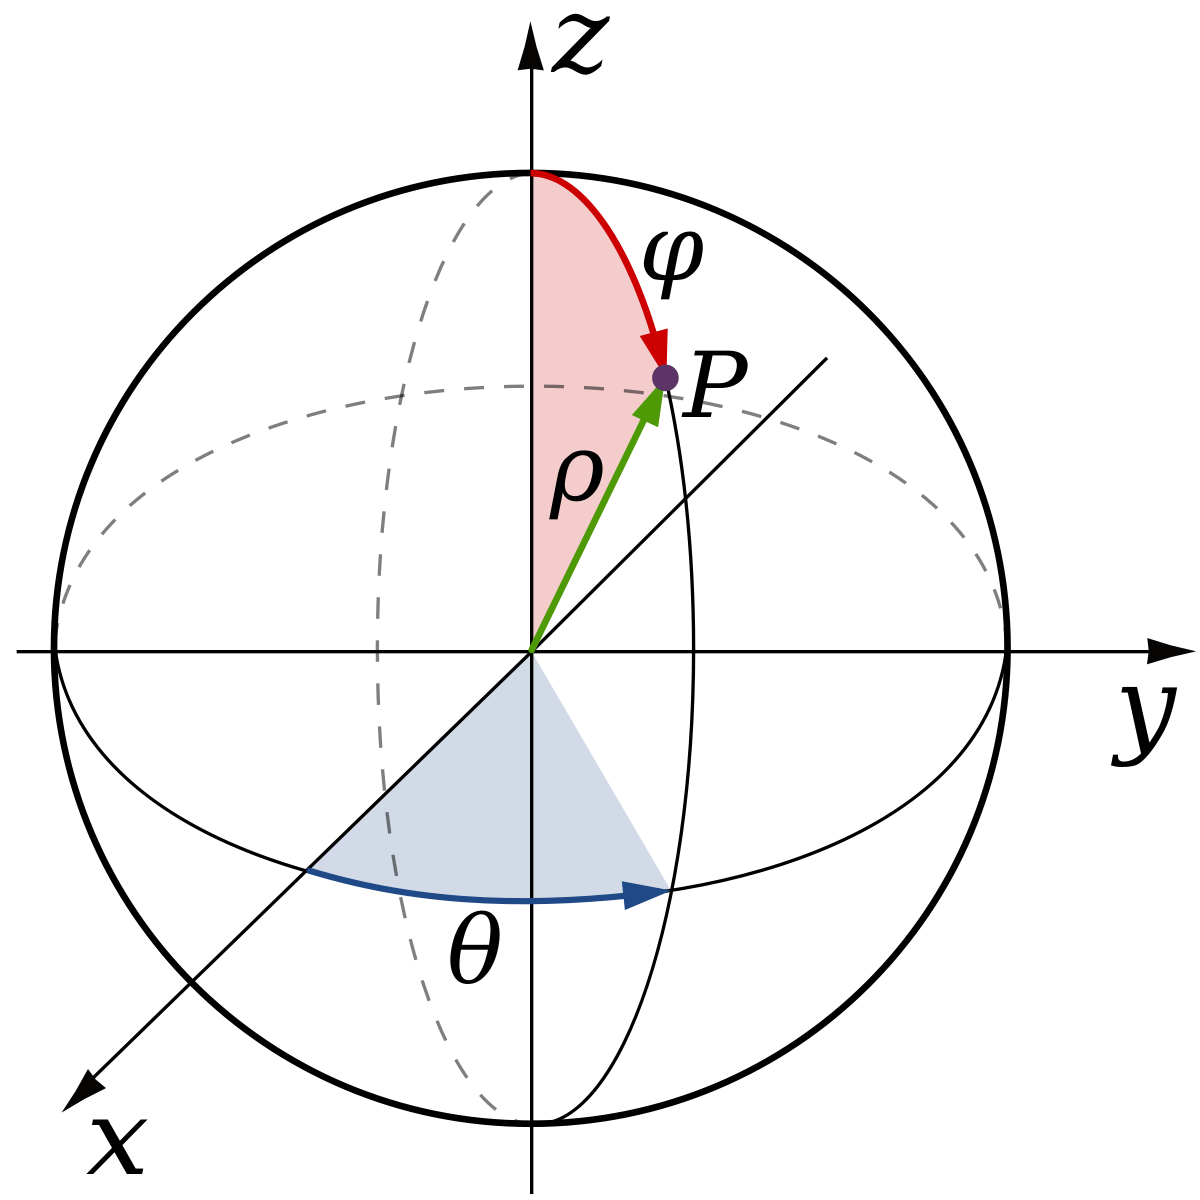
\includegraphics[height=0.4\textheight]{Image/sphere.png}
    \caption{Spherical coordinate representation.}
    \label{SC1}
\end{figure}
To obtain the time between the initial flash and the scanning, the algorithm will start a timer after the flash. And it will acquire the time when the scalar product between the LightHouse-Object vector (that is only known by the algorithm) and the normal vector is the smallest, since the normal vector changes with time. A zero scalar product means that the object is in the scanning plan, since that exact moment cannot be detected, taking the smallest value is a good approximation of that moment. After that step, we can easily get the angles with a simple cross product, since we know the time of a full scanning.
\begin{equation}
\label{angle_calculus}
    \theta~=~\displaystyle\frac{\tau~\pi}{T}
\end{equation} where $\theta$ is the angle as it can be seen in figure [\ref{SC1}], $\tau$ the acquired time and $T$ the time for a full scanning (that is eqaul to $8.333 \mu s$ as seen before). After the obtaining of the four angles, by using the spherical coordinate obtained with [\ref{spherique}], the vector LightHouse-object can be obtained. Then, since the position and the orientation of the lighthouses is known, the algorithm can compute the localization of the object in the room.
    $$x~=~sin(\phi)cos(\theta)$$
\begin{equation}
\label{spherique}
    y~=~sin(\phi)~sin(\theta)
    \end{equation}
    $$z~=sin((\phi)$$
The vector LightHouse-object is first defined in the Lighthouse landmark, but is then returned in the world landmark by doing the same rotation and translation the lighthouse had for it to be in its actual position. Doing this transformation ensure that every value given is in the world landmark, witch will eliminate any source of confusion about the position. Technically, this had to be done with the calibration of the lighthouses between them, but in the simulation, the rotation is known from the beginning (same thing for the translation).
\subsection{Object localization from photo-diode}
\label{Obj}
Localizing the object in 3D space with this method ends up with the calculus of the point of intersection of two lines. From the previous data, the problem can be seen as two points (Position of the LightHouses) and two vectors (the Lighthouse-object vector obtained thanks to the angles by using [\ref{angle_calculus}] and [\ref{spherique}]). From two points and vector: two lines. From two lines: one point that will be the position of the object. \newline
However, if in the theory this point exist exactly, it is really rare that two lines intersect in a 3D space. And since the scanning moment is approximated, the intersection point will be approximated too. The trick to compute this non-existent point is to find a third line that is perpendicular to the two lines. The intersection point will then be the middle of this line (see figure[\ref{inter}]).
\begin{figure}
\centering
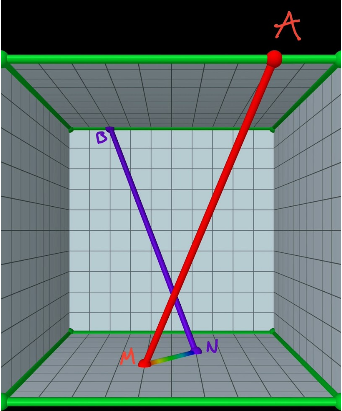
\includegraphics[width=1.0\columnwidth]{Image/interscetion.png}
\caption{Non-existent intersection point trick where $A$ and $B$ are the two lightHouses and $MN$ the perpendicular line. \cite{cedric}}
\label{inter}
\end{figure}
Let $A$ and $B$ be the lighthouse coordinate and $u$ and $v$ their respectiv LightHouse-object vector. The two lines that come from these values (the red nand the blue in [\ref{inter}]) are represented by:
$$ A  + \lambda u $$ and $$B + \nu v$$ with $\lambda,\nu \in R$. 
The points $M$ and $N$ are characterized by the fact that the vector $MN$ is orthogonal to the two starting lines, or, equivalently, to the vectors u and v. To calculate them, we can write $M~=~A~+~\lamda~u$ and $N~=~ B ~+~ \nu~v$ so that $MN~=~ AB~+~ \nu v~-~\lambda u$. The two orthogonality conditions with the scalar product are:
$$<MN,u> = 0$$
$$<MN,v> = 0
$$
There is then two equation with two unknown that are $\lambda$ and $\nu$. Since the middle of the $MN$ is the most representative point for this probleme, the coordinate $I$ that represents the estimated position of the object will be:

$$
 I ~=~[ (a1 ~+ ~b1~ +~ \lambda u1 ~+~ \nu v1) / 2~ ,~   (a2 + b2 + \lambda u2 + \nu v2) / 2 ~,$$
 $$~ (a3~ +~ b3~ +~ \lambda u3 ~+~ \nu v3) / 2 ]
 $$
 
 \subsection{Object localization from the acceleration}
 The results obtained from the photo-diode is precised but takes too much time, a total of $35 \mu s $ to get the complete position of the object. To be able to estimate the position of the object in this time-lapse, the acceleration can be obtained by deriving twice the position obtained thanks to the photo-diodes and estimate the position of the object with it while it get the precise value of the position given again by the photo-diode. This position is obtained at each time by integrating it twice. Figure [\ref{axel}] shows how this method works.
 \begin{figure}
 \centering
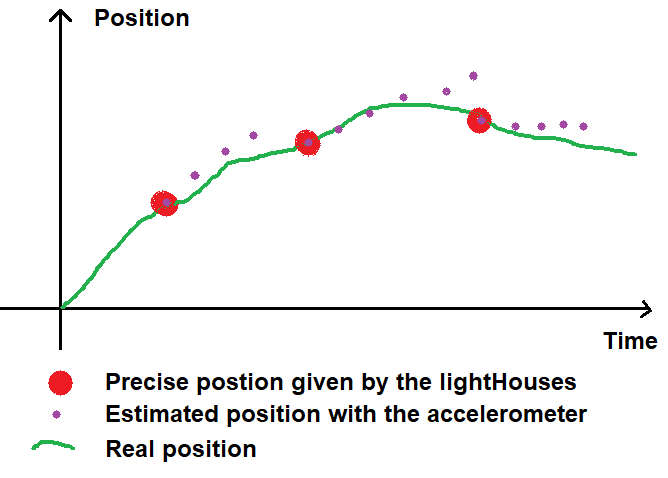
\includegraphics[width=1.0\columnwidth]{Image/axel.png}
\caption{Estimated position with the accelerometer and the photo-diode throw time. While the algorithm waits for the precise position of the object, it compute it with the values of the accelerometer}
\label{axel}
\end{figure}
\section{Results}

In this section we will show you the results obtained with our algorithm. We used OpenFramework for the GUI. Since the simulation of $35 \mu s $ won't allow us to see anything, a full positioning is done in 10 seconds. Figure [\ref{g1}] and [\ref{g2}] shows the simulated world, on the top corner we can see the two lighthouses, the colored balls around it are the normal vector of the plan that we mentioned in section 4.1 and the two balls in the box are the true position (white ball) and the estimated position (blue ball). There are also other values of the dimension of the box and the exact position of the two balls. We can see that estimated position is really close to the real position. However, the more far we go from the lighthouses, the less precise it became.
 \begin{figure}
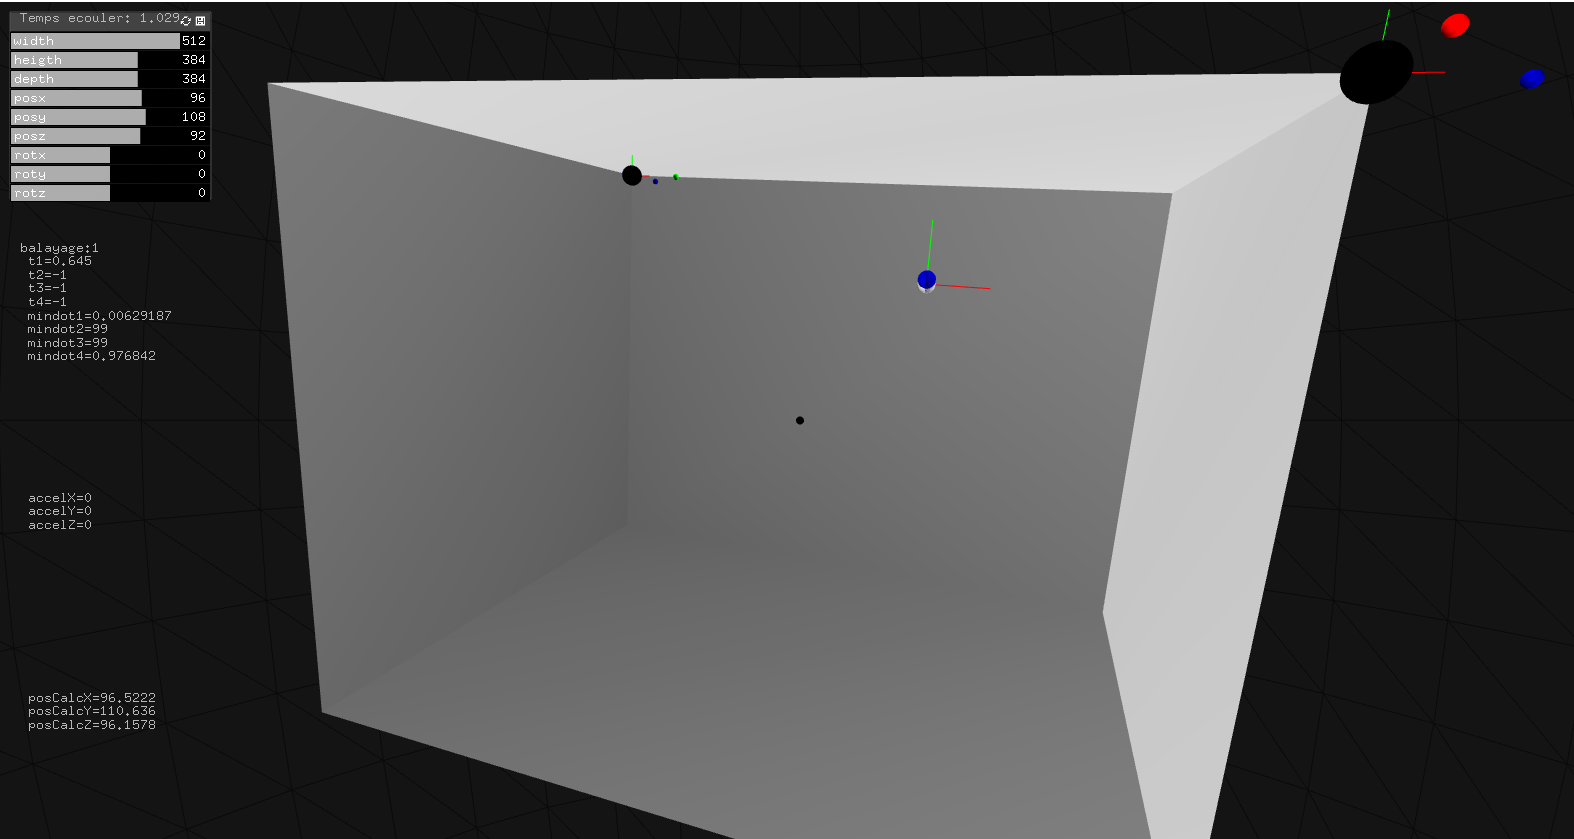
\includegraphics[width=1.0\columnwidth]{Image/GUI2.png}
\caption{Simulation of the room, where the white ball represents the exact position of the object and the blue one its estimated position with the lighthouse.}
\label{g1}
\end{figure}

 \begin{figure}
 \centering
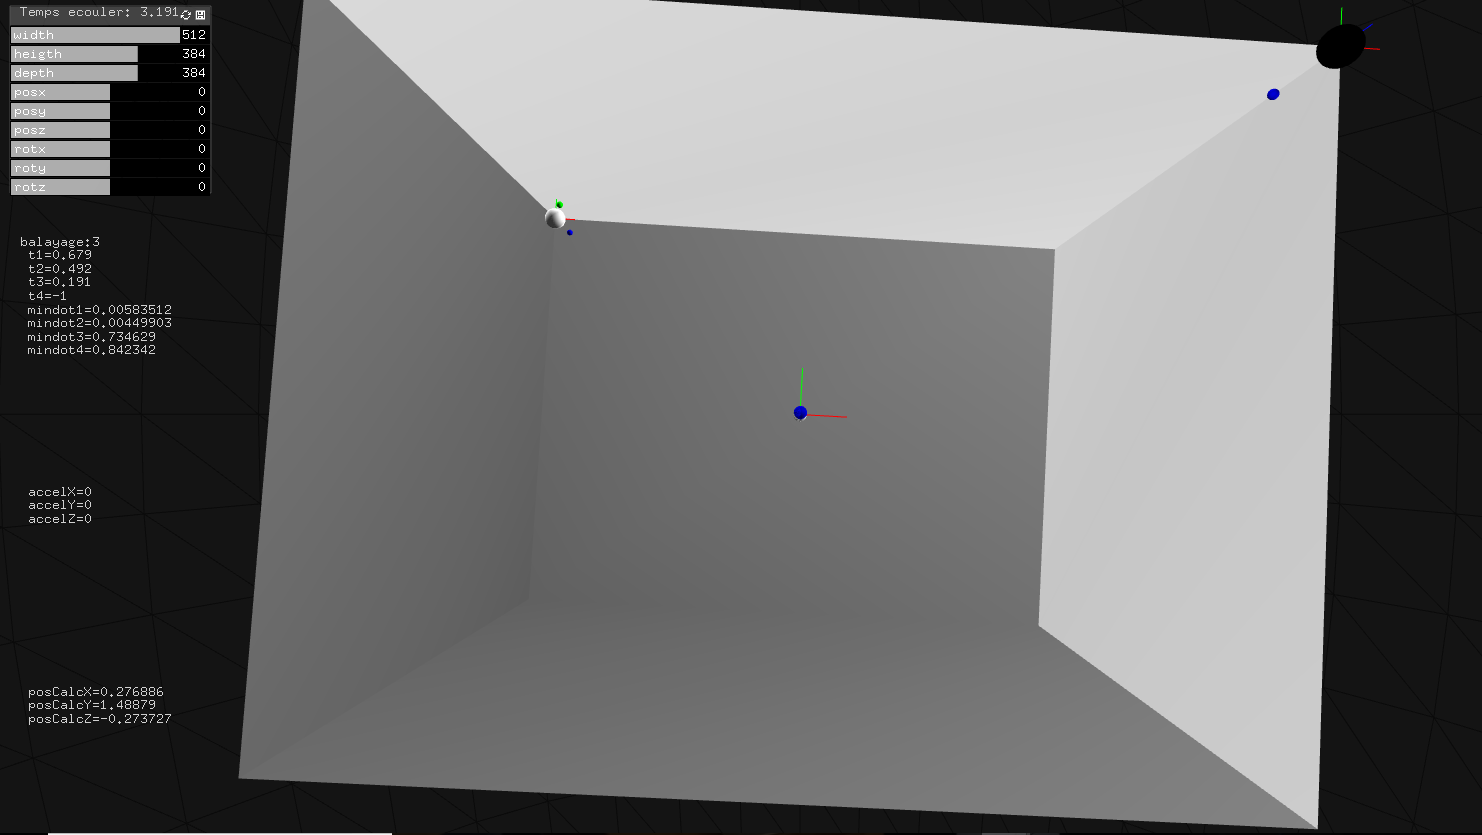
\includegraphics[width=1.0\columnwidth]{Image/GUI1.png}
\caption{Simulation of the room, where the white ball represents the exact position of the object and the blue one its estimated position with the lighthouse.}
\label{g2}
\end{figure}

As said before, time is a critical value for this method. The function to obtain the time is $getTime$ which gets the time from the computer. Thus, the value obtained is never the same for the exact same position. It means that the precision of the simulation depends directly on the power of calculus of the computer. If we want to simulate the whole position computing in 1 second, the results will be really bad. \newline
This imprecision leads to another imprecision that we mentioned before. Indeed, we cannot get exactly the moment that the scanning plan pass throw the object and the scalar product between the LightHouse-object vector and the normal to the plan vector will most likely never be obtained at its true values (see figure [\ref{scal}]).

 \begin{figure}
 \centering
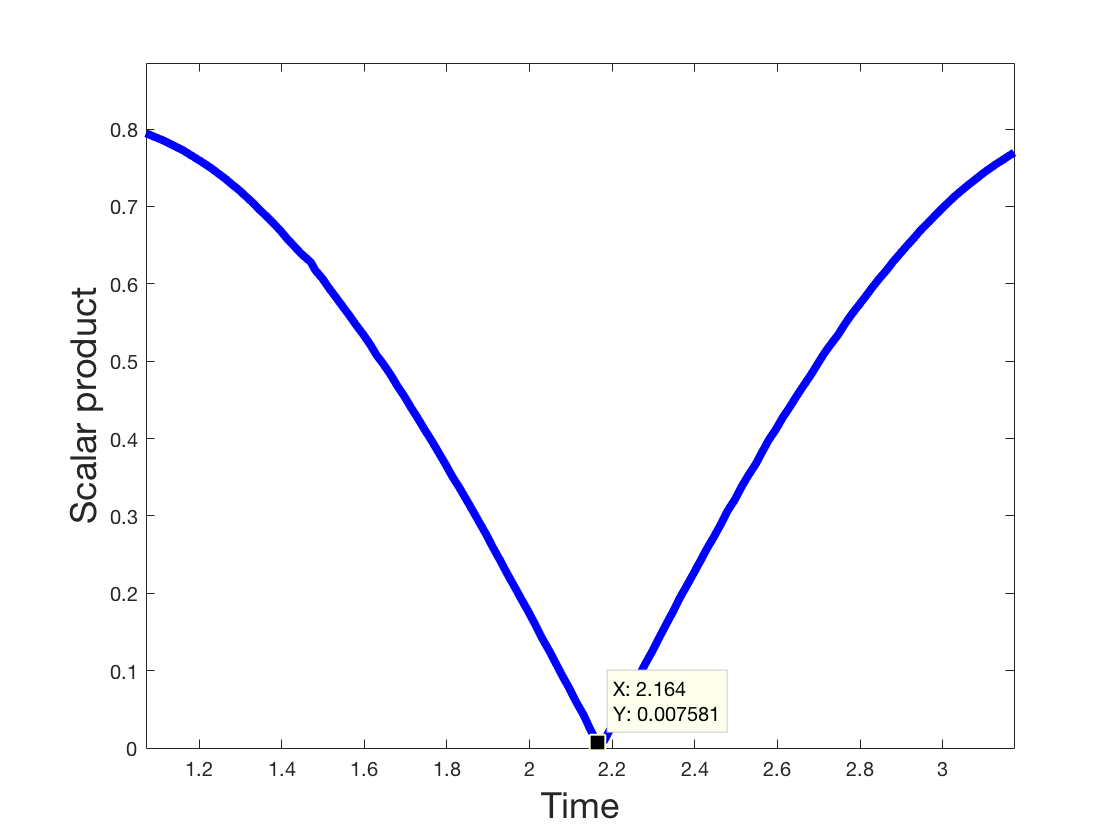
\includegraphics[width=1.0\columnwidth]{Image/scalaire.png}
\caption{Evolution of the scalar product between the LightHouse-object vector and the normal to the plan vector throw time, in a case where the object is around the middle of the room}
\label{scal}
\end{figure}

At this step, we have a precise but slow 3D positioning. We now wants to use the Kalman Filter introduced to you in section 3. Figure below show a typical response of each sensors and of the kalman filter : \\

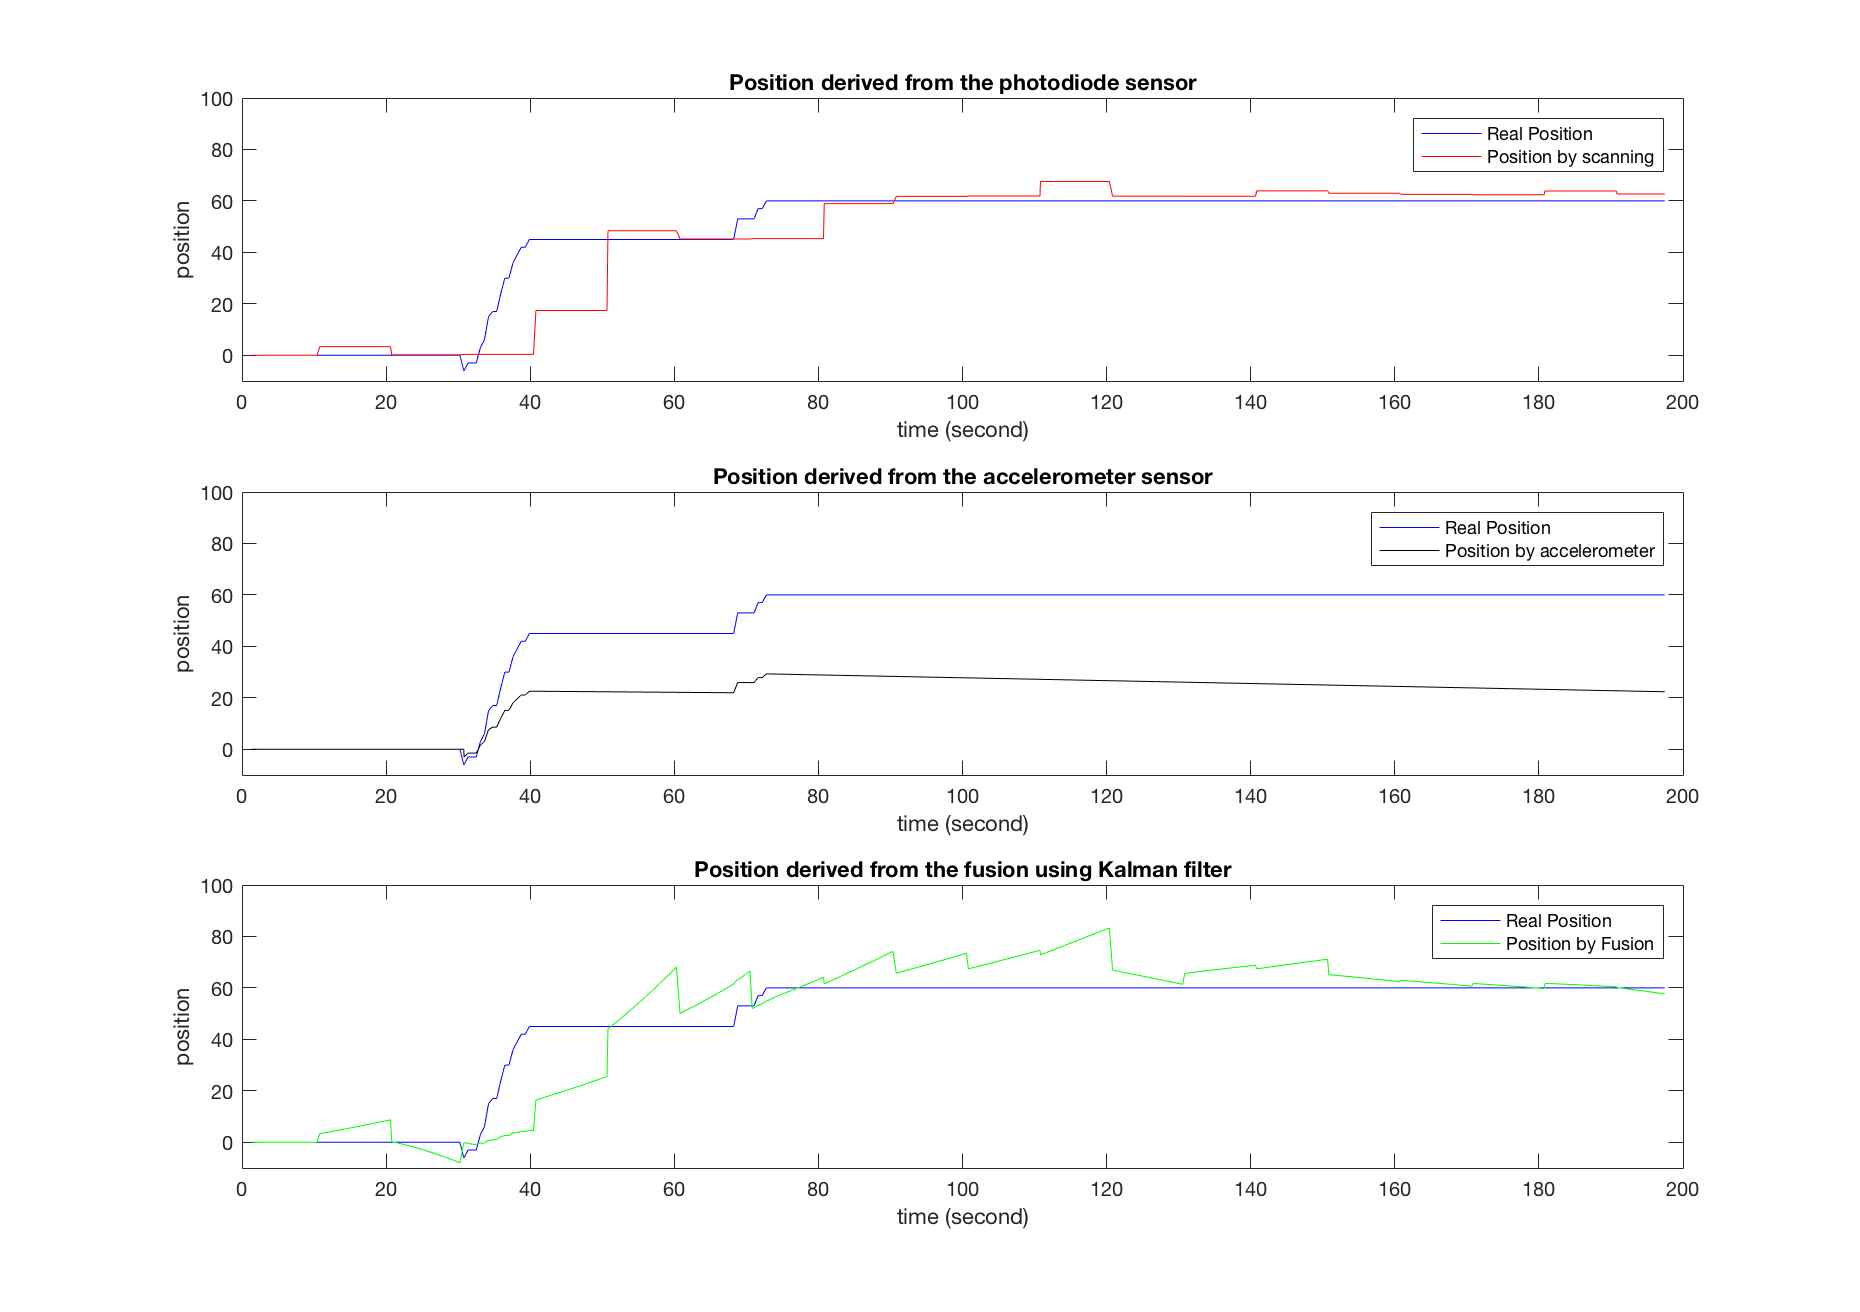
\includegraphics[width=1.0\columnwidth]{Image/graphes2.png}

We can see that the kalman filter response worse than the scan response. That is due to a bad tuning of the Kalman filter because of the lack of time. However, we can see as expected that the position derived from the photo-diode sensor is precise but slow. We can expect good prospects for improvement with a better tunning of the filter. Above all, the Kalman filter will be easier to tune as the GUI is now easy to use. 



% The following two commands are all you need in the
% initial runs of your .tex file to
% produce the bibliography for the citations in your paper.
\bibliographystyle{abbrv}
\bibliography{vldb_sample}  % vldb_sample.bib is the name of the Bibliography in this case
% You must have a proper ".bib" file
%  and remember to run:
% latex bibtex latex latex
% to resolve all references



%APPENDIX is optional.
% ****************** APPENDIX **************************************
% Example of an appendix; typically would start on a new page
%pagebreak



\end{document}
